% ****** Start of file apssamp.tex ******
%
%   This file is part of the APS files in the REVTeX 4.2 distribution.
%   Version 4.2a of REVTeX, December 2014
%
%   Copyright (c) 2014 The American Physical Society.
%
%   See the REVTeX 4 README file for restrictions and more information.
%
% TeX'ing this file requires that you have AMS-LaTeX 2.0 installed
% as well as the rest of the prerequisites for REVTeX 4.2
%
% See the REVTeX 4 README file
% It also requires running BibTeX. The commands are as follows:
%
%  1)  latex apssamp.tex
%  2)  bibtex apssamp
%  3)  latex apssamp.tex
%  4)  latex apssamp.tex
%
\documentclass[%
 reprint,
superscriptaddress,
%groupedaddress,
%unsortedaddress,
%runinaddress,
%frontmatterverbose, 
%preprint,
%preprintnumbers,
%nofootinbib,
%nobibnotes,
%bibnotes,
 amsmath,amssymb,
aps,
% prl,
%prb,
%rmp,
%prstab,
%prstper,
%floatfix,
]{revtex4-2}

\usepackage{xcolor}

\definecolor{codegreen}{rgb}{0,0.6,0}
\definecolor{codegray}{rgb}{0.5,0.5,0.5}
\definecolor{codepurple}{rgb}{0.58,0,0.82}
\definecolor{backcolour}{rgb}{0.95,0.95,0.92}
\definecolor{urlblue}{HTML}{007bff}

\usepackage{graphicx}% Include figure files
\usepackage{dcolumn}% Align table columns on decimal point
\usepackage{bm}% bold math
\usepackage{orcidlink}
\usepackage{hyperref}% add hypertext capabilities
\usepackage{cleveref}

\newcommand{\Tr}{\ensuremath{\textup{Tr}}}
\renewcommand{\bf}[1]{\ensuremath{\textbf{#1}}}

% \usepackage{caption} % These break revtex figure captions, please don't use.
% \usepackage{subcaption}


\hypersetup{
    colorlinks = true,
    linkcolor  = urlblue,
    citecolor  = urlblue,
    urlcolor   = urlblue,
}

\urlstyle{same}

\bibliographystyle{apsrev4-2}

\usepackage[mathlines]{lineno}% Enable numbering of text and display math
% \linenumbers\relax % Commence numbering lines

%\usepackage[showframe,%Uncomment any one of the following lines to test 
%%scale=0.7, marginratio={1:1, 2:3}, ignoreall,% default settings
%%text={7in,10in},centering,
%%margin=1.5in,
%%total={6.5in,8.75in}, top=1.2in, left=0.9in, includefoot,
%%height=10in,a5paper,hmargin={3cm,0.8in},
%]{geometry}

\begin{document}

\preprint{APS/123-QED}

\title{An exact chiral amorphous spin liquid}


\author{G. Cassella \orcidlink{0000-0003-4506-5791}}
\thanks{These three authors contributed equally, and names are ordered alphabetically.}
\affiliation{\small Blackett Laboratory, Imperial College London, London SW7 2AZ, United Kingdom}


\author{P. D'Ornellas \orcidlink{0000-0002-2349-0044}}
\thanks{These three authors contributed equally, and names are ordered alphabetically.}
\affiliation{\small Blackett Laboratory, Imperial College London, London SW7 2AZ, United Kingdom}


\author{T. Hodson \orcidlink{0000-0002-4121-4772}}
\thanks{These three authors contributed equally, and names are ordered alphabetically.}
\affiliation{\small Blackett Laboratory, Imperial College London, London SW7 2AZ, United Kingdom}

\author{W. M. H. Natori \orcidlink{0000-0002-0740-2956}}
\affiliation{Institut Laue-Langevin, BP 156, 41 Avenue des Martyrs, 38042 Grenoble Cedex 9, France}

\author{J. Knolle \orcidlink{0000-0002-0956-2419}}
\affiliation{\small Blackett Laboratory, Imperial College London, London SW7 2AZ, United Kingdom}
\affiliation{Department of Physics TQM, Technische Universit{\"a}t M{\"u}nchen, James-Franck-Stra{\ss}e 1, D-85748 Garching, Germany}
\affiliation{Munich Center for Quantum Science and Technology (MCQST), 80799 Munich, Germany}

%at the end Global choices we need to make
% either vortex or flux sectors
% use either pointset or set of points


\date{\today}

\begin{abstract}
filler filler filler filler filler filler filler filler filler filler filler filler filler filler filler filler filler filler filler filler filler filler filler filler filler filler filler filler filler filler filler filler filler filler filler filler filler filler filler filler filler filler filler filler filler filler filler filler filler filler filler filler filler filler filler filler filler filler filler filler filler filler filler filler filler filler filler filler filler filler filler filler filler filler filler filler filler filler filler filler filler filler filler filler filler filler filler filler filler filler filler filler filler filler filler filler filler filler filler filler filler filler filler filler filler filler filler filler filler filler filler filler filler filler filler filler filler filler filler filler filler filler filler filler filler filler filler filler filler filler filler filler filler filler filler filler filler filler filler filler filler filler filler filler filler filler filler filler filler filler filler filler filler filler filler filler filler filler filler filler filler filler filler filler filler filler filler filler filler filler filler filler filler filler filler filler filler filler filler filler filler filler filler filler filler filler filler filler filler filler filler filler filler filler filler filler filler filler filler filler filler filler filler filler filler filler filler filler filler filler 
\end{abstract}


\maketitle




\begin{figure*}[ht!]
    \centering
    \includegraphics[width=1.\textwidth]{figs/figure_1.pdf}
    \caption{\textbf{(a)} Amorphous lattice generated via Voronoi tessellation of a uniformly distributed random point set on the unit square. Periodic boundary conditions are imposed by tiling the unit square before Voronoi tessellation. \textbf{(b)} Magnified portion of the amorphous lattice. Arrows from site $j$ to site $k$ indicate the bond variable $u_{jk} = 1$ while $u_{kj} = -1$. Shading of the plaquettes indicates the $\mathbb{Z}_2$ flux $\phi_p = +1$ ($-1$) through white (grey) plaquettes. Colors correspond to a valid assignment of the bond colourings, $\alpha_{jk}$. The inset demonstrates the Majorana construction on a tri-coordinate motif, which allows for the exact solution of the model. \textbf{(c)} Phase diagram of the amorphous Kitaev model with varying exchange coupling. The isotropic regime $|J_x| \approx |J_y| \approx |J_z|$ (B), exhibits a topologically non-trivial chiral QSL ground state with Chern number $\nu=\pm1$. The Fermion gap of the ground state flux sector closes at the phase boundary (solid black lines), and a topological phase transition occurs to a trivial $\nu=0$ phase (A) in the anisotropic coupling regime. This phase boundary was obtained by averaging over 20 amorphous lattice realisations with $\sim400$ sites. Dotted black lines indicate the corresponding phase boundaries in the Kitaev honeycomb model.}
    \label{fig:example_lattice}
\end{figure*}

Amorphous materials are glassy condensed matter systems characterised by short-range constraints in the absence of long-range crystalline order as first studied in amorphous semiconductors~\cite{Yonezawa1983,zallen2008physics}. In general, the bonds of a whole range of covalent compounds enforce local constraints around each ion, e.g.~a fixed coordination number $z$, which has enabled the prediction of energy gaps even in lattices without translational symmetry~\cite{Weaire1976,gaskell1979structure}, the most famous example being amorphous Ge and Si with $z=4$~\cite{Weaire1971,betteridge1973possible}. Recently, following the discovery of topological insulators (TIs) it has been shown that similar phases can exist in amorphous systems characterized by protected edge states and topological bulk invariants~\cite{mitchellAmorphousTopologicalInsulators2018,agarwala2019topological,marsalTopologicalWeaireThorpeModels2020,costa2019toward,agarwala2020higher,spring2021amorphous,corbae2019evidence}. However, research on electronic systems has been mostly focused on non-interacting systems with a few notable exceptions for understanding the occurrence of superconductivity~\cite{buckel1954einfluss,mcmillan1981electron,bergmann1976amorphous} {\bf JK: CECK OLD EMAIL WITH THEORY WORKS} in amorphous materials and recently the effect of strong repulsion in amorphous TIs~\cite{kim2022fractionalization}.         




Magnetic phases in amorphous systems have been investigated since the 1960s, mostly through the adaptation of theoretical tools developed for disordered systems \cite{aharony1975critical,Petrakovski1981,kaneyoshi1992introduction,Kaneyoshi2018} and numerical methods~\cite{fahnle1984monte,plascak2000ising}. Research focused on classical Heisenberg and Ising models which have been shown to account for observed behavior of ferromagnetism, disordered antiferromagnetism and widely observed spin glass behaviour~\cite{coey1978amorphous}. However, the role of spin-anisotropic interactions and quantum effects has not been addressed. Similarly, it is an open question whether magnetic frustration in amorphous quantum magnets can give rise to long-range entangled quantum spin liquid (QSL) phases. 


%Broad constraints to the possible phases hosted by Heisenberg amorphous magnets were provided by the phenomenological theory developed by Andreev and Marchenko \cite{Andreev1,Andreev2,Andreev3}. The phases in this theory are described by a set of macroscopic magnetic vectors that transform according to the irreducible representations of the group of spatial symmetries of the system \cite{Andreev1}. Amorphous magnets are treated, on average, as homogeneous and isotropic, being thus symmetric under three-dimensional rotations and spatial inversion \cite{Andreev2}. Only three types of phases are consistent to this group of symmetries, corresponding to ferromagnets, disordered antiferromagnets, or spin glasses \cite{Andreev2,Andreev3}.

\par
Two intentional simplifications of Andreev's and Marchenko's theory were the neglect of spin-orbit coupling induced anisotropies and the effects arising from the local structure of amorphous lattices. It is then expected that their theory is invalid for amorphous compounds generated from crystalline magnets with strong spin-orbit coupling with tight geometrical arrangements. Several instances of these magnets were synthesized in the last decade, among which we highlight the Kitaev materials \cite{Jackeli2009,HerrmannsAnRev2018,Winter2017,TrebstPhysRep2022,Takagi2019}. It was suggested (and later observed) that heavy-ion Mott insulators formed by edge-sharing octahedra could be good platforms for the celebrated Kitaev model on the honeycomb lattice \cite{Jackeli2009}, an exactly solvable model whose ground state is a quantum spin liquid (QSL)~\cite{Anderson1973,Knolle2019,Savary2016,Lacroix2011} characterized by a static $\mathbb Z_2$ gauge field and Majorana fermion excitations \cite{kitaevAnyonsExactlySolved2006}. The model displays bond-dependent Ising-like exchanges that give rise to local symmetries, which are essential to its mapping onto a free fermion problem \cite{Baskaran2007,Baskaran2008}. Such a mapping is rigorously extendable to any three-coordinated graph in two or three dimensions satisfying a simple geometrical condition \cite{Nussinov2009,OBrienPRB2016, yaoExactChiralSpin2007,Peri2020}. Thus, it reasonable to suppose that the Kitaev model is also analytically treatable on certain amorphous lattices, therefore becoming a realistic starting point to study the overlooked possibility of QSLs in amorphous magnets. \par
In this letter, we study Kitaev spin liquids (KSLs) stabilized by the $S=1/2$ Kitaev model \cite{kitaevAnyonsExactlySolved2006} on coordination number $z=3$ random networks generated via Voronoi tessellation \cite{mitchellAmorphousTopologicalInsulators2018,marsalTopologicalWeaireThorpeModels2020}. On these lattices, the KSLs generically break time-reversal symmetry (TRS), as expected for any Majorana QSL in graphs containing odd-sided plaquettes \cite{Chua2011,ChuaPRB2011,Fiete2012,Natori2016,Wu2009, WangHaoranPRB2021}. An extensive numerical study showed that the $\mathbb Z_2$ gauge fluxes on the ground state can be described by a conjecture consistent with Lieb's theorem \cite{lieb_flux_1994}. In contrast to the honeycomb case, the amorphous KSLs are gapless only along certain critical lines. These manifolds separate two gapped KSLs that are topologically differentiated by a local Chern number $\nu$ \cite{peru_preprint, mitchellAmorphousTopologicalInsulators2018} in analogy with the KSLs on the decorated honeycomb lattice \cite{yaoExactChiralSpin2007}. The $\nu=0$ phase is the amorphous analogue of the abelian toric-code QSL \cite{kitaev_fault-tolerant_2003}, whereas the $\nu=\pm1$ KSLs is a non-Abelian chiral spin liquid (CSL). We study two specific features of the latter liquid: topologically protected edge states and a thermal-induced Anderson transition to a thermal metal phase \cite{selfThermallyInducedMetallic2019}. \par


% The Kitaev spin liquids are classified by their Majorana fermion dispersion and topological properties. On the honeycomb lattice, tuning the exchange couplings $J^\alpha$ can change the ground state from a gapped QSL with Abelian anyonic excitations (e.g., when $J^z\gg J^x,J^y$) or gapless (e.g., when $J^z=J^x=J^y$). In the latter case, breaking time reversal symmetry (TRS) opens a gap that signals the onset of a chiral spin liquid (CSL) phase supporting non-Abelian excitations and protected edge modes. On the honeycomb lattice, CSLs are only obtained by perturbing a Hamiltonian with, for example, magnetic fields \cite{kitaevAnyonsExactlySolved2006} or Dzyaloshinskii-Moriya exchanges \cite{Ralko2020}. CSLs on the pure Kitaev model can be obtained on $z=3$ lattices containing odd-sided plaquettes, for which any Majorana QSL displays spontaneous TRS breaking \cite{Chua2011,ChuaPRB2011,Fiete2012,Natori2016,Wu2009, WangHaoranPRB2021}, as confirmed on decorated honeycomb \cite{yaoExactChiralSpin2007} and non-Archimedean \cite{Peri2020} lattices.


{\it The Model ---} 
We start with a brief review of the Kitaev model on the honeycomb lattice \cite{kitaevAnyonsExactlySolved2006}. Here, a spin-1/2 is placed on every vertex and each bond is labelled by an index $\alpha \in \{ x, y, z\}$. The bonds are arranged such that each vertex connects to exactly one bond of each type. The Hamiltonian is given by
\begin{equation}
    \label{eqn:kitham}
    \mathcal{H} =  - \sum_{\langle j,k\rangle_\alpha} J^{\alpha}\sigma_j^{\alpha}\sigma_k^{\alpha},
\end{equation}
where $\sigma^\alpha_j$ is a Pauli matrix acting on site $j$, \(\langle j,k\rangle_\alpha\) is a pair of nearest-neighbour indices connected by an $\alpha$-bond with exchange coupling $J^\alpha$. For each plaquette of the lattice, we can define the conserved operator $ W_p = \prod \sigma_j^{\alpha}\sigma_k^{\alpha}$, where the product runs clockwise over the bonds around the plaquette. This provides an extensive number of conserved plaquettes that allow us to split the Hilbert space in terms of the eigenvalues of $W_p$.\par
The KSL is uncovered by transforming eqn.~\ref{eqn:kitham} to a four-Majorana representation of the spin operators, $\sigma_i^\alpha = i b_i^\alpha c_i$ \cite{kitaevAnyonsExactlySolved2006}, where the Hamiltonian takes the form
\begin{equation}\label{eqn:majorana_hamiltonian}
    \mathcal{H} = \frac{i}{4}\sum_{j,k}A_{jk}^{(\alpha)}c_jc_k.
\end{equation}
Here, $A_{jk}^{(\alpha)}=2J^{\alpha}u_{jk}$ with $\hat u_{jk} = ib_j^{\alpha}b_k^{\alpha}$ being conserved $\mathbb Z_2$ bond operators. Once the $\hat u_{jk}$ eigenvalues are fixed, the Kitaev model becomes equivalent to a fermionic problem that can be diagonalized with standard methods \cite{BlaizotRipka1986}. \par
The Kitaev Hamiltonian remains exactly solvable on any graph in which no site connects to more than one bond of the same type \cite{Nussinov2009}. Thus, we are  restricted to lattices in which every vertex has coordination number $z \leq 3$. Here, such graphs are generated with Voronoi tessellation \cite{florescu_designer_2009}. A set of points are sampled uniformly from the unit square and cells are generated as the region of space closer to a given point than any other. The lattice is given by the boundaries between cells with edges at the interface of two cells and vertices at the point where three edges meet. Periodic boundary conditions are imposed by tiling the initial set of points and then connecting corresponding edges that cross the unit square boundaries - see \cref{apx:lattice_construction} for technical details. One example of such an amorphous lattice is shown in~\cref{fig:example_lattice}(a).\par
Once a random network has been generated, the bonds types must be assigned in a way that is consistent with our condition, which we refer to as a \textit{three-edge colouring}. The problem of finding such a colouring was shown to be equivalent to the classical problem of four-colouring the faces, which is always solvable in planar graphs~\cite{Tait1880, appelEveryPlanarMap1989a}. On the torus, a face colouring can require up to seven colours \cite{ringel_solution_1968}, and so not all graphs can be assumed to be 3-edge colourable. However, such exceptions are rare -- every graph generated in this study admitted multiple distinct 3-edge colourings. The problem of finding a colouring for a given graph can be reduced to a Boolean satisfiability problem \cite{Karp1972}, which we then solve using the open-source solver \texttt{MiniSAT}~\cite{imms-sat18}. \par
Once the three-edge colouring has been found, the Kitaev Hamiltonian is mapped onto eqn.~\ref{eqn:majorana_hamiltonian}, which corresponds to the spin fractionalization in terms of a static $\mathbb Z_2$ gauge fields and $c$ matter as indicated in ~\cref{fig:example_lattice}(b) \cite{Baskaran2007}.  Strictly speaking, the Majorana system is equivalent to the original spin system after applying a projector operator \cite{pedrocchiPhysicalSolutionsKitaev2011,Zschocke_Physical_states2015,selfThermallyInducedMetallic2019}, whose form is presented in \cref{apx:projector}. Despite this caveat, one can still use eqn.~\ref{eqn:majorana_hamiltonian} to evaluate the expectation values of operators conserving $\hat u_{jk}$ in the thermodynamic limit \cite{Yao2009,knolle_dynamics_2016}. This type of operator is exemplified by the Hamiltonian itself, for which the ground state energy of a fixed sector is the sum of the negative eigenvalues of $iA/4$ in eqn.~\ref{eqn:majorana_hamiltonian}, and whose excitations are extracted from the positive eigenvalues of the same matrix. 

{\it Fluxes and the Ground State --- } 
Let us now consider the conserved operators $ W_p = \prod \sigma_j^{\alpha}\sigma_k^{\alpha}$ on amorphous lattices. When represented in the Majorana Hilbert space, these operators correspond to ordered products of $\hat u_{jk}$, and their fixed eigenvalues are written as
\begin{equation} \label{eqn:flux_definition}
    \phi_p = \prod_{(j,k) \in \partial p} (-iu_{jk}),
\end{equation}
where the pairs $j,k$ are crossed around the border $\partial p$ of the plaquette on the \textit{clockwise} orientation. In periodic boundaries there is an additional  pair of global $\mathbb{Z}_2$ fluxes $\Phi_x$ and $\Phi_y$, which are calculated along an arbitrary closed path that wraps the torus in the $x$ and $y$ directions respectively. The energy difference between distinct flux sectors decays exponentially with system size, so that the ground state of any flux sector in the thermodynamic limit displays a fourfold topological degeneracy \cite{kitaev_fault-tolerant_2003}. \par
We now need to determine the ground state flux sectors. First, let us recall that Majorana QSLs emerging on graphs containing odd-sided plaquette undergo a spontaneous TRS breaking \cite{Chua2011,yaoExactChiralSpin2007,ChuaPRB2011,Fiete2012,Natori2016,Wu2009,Peri2020, WangHaoranPRB2021}. Therefore, there will be always a twofold ground state degeneracy due to time-reversal, in which one ground state is related to the other by inversion of imaginary $\phi_p$ fluxes \cite{yaoExactChiralSpin2007}. An insight pointing to the ground state sectors come from the model on the honeycomb lattice, for which a theorem proved by Lieb sets that the ground state sector to be $\phi_p=+1$, $\forall p$ \cite{lieb_flux_1994}. Although Lieb's theorem is not extendable to amorphous lattices, it is suggested the ground state energy for a sufficiently large system is minimised by setting \cite{OBrienPRB2016}
\begin{align} \label{eqn:gnd_flux}
    \phi_p^{\textup{g.s.}} = -(\pm i)^{n_{\textup{sides}}},
\end{align}
where $n_{\textup{sides}}$ is the number of edges that form $p$ and the global choice of the sign of $i$ gives each of the two TRS-degenerate ground state flux sectors. Such a conjecture is consistent with Lieb's theorem on regular lattices \cite{lieb_flux_1994} and is supported by numerical evidence as detailed in \cref{apx:ground_state}. Once we have identified the ground state, any other sector can be characterized by the configuration of vortices, i.e. by the plaquettes whose flux is flipped with respect to $\left\{\phi_p^{\textup{g.s.}}\right\}$.\par

\begin{figure}
    \centering
    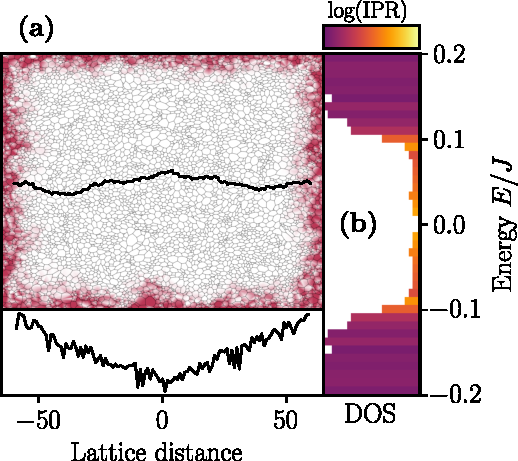
\includegraphics[width=\columnwidth]{figs/figure_2_bashed}
    \caption{\textbf{(a)} In-gap fermionic wavefunction drawn from the ground state flux sector in open boundary conditions, showing the state corresponds to a topological edge mode. Cut of the density along a line of lattice sites spanning the system (black line) is shown in the bottom subfigure on a logarithmic scale, demonstrating the characteristic exponential decay of topological edge modes with distance from the system edge. \textbf{(b)} Ground-state flux sector fermionic density of states in open boundary conditions, colored by inverse participation ratio. The increased inverse participation ratio of the in-gap states signifies their localisation to the edges of the system.}
    \label{fig:edge_modes}
\end{figure}

{\it Chern Number and Edge Modes ---} 
We numerically found that the amorphous KSLs are generally gapped, except along the critical lines displayed in \ref{fig:example_lattice}(c). The QSLs separated by these lines are distinguished by a real-space analogue of the Chern number \cite{bianco_mapping_2011,Hastings_Almost_2010}. A similar topological number was discussed by Kitaev on the honeycomb lattice  \cite{kitaevAnyonsExactlySolved2006} that we shall use here with a slight modification \cite{peru_preprint, mitchellAmorphousTopologicalInsulators2018}. For a choice of flux sector, we calculate the projector $P$ onto the negative energy eigenstates of the matrix $iA$ defined in eqn.~\ref{eqn:majorana_hamiltonian}. The local Chern number around a point $\bf R$ in the bulk is given by 
\begin{align}
    \nu (\bf R) = 4\pi \Im \Tr_{\textup{Bulk}} 
    \left ( 
    P\theta_{R_x} P \theta_{R_y} P
    \right ),
\end{align}
where $\theta_{R_x}$ is a step function in the $x$-direction, with the step located at $x = R_x$, $\theta_{R_y}$ is defined analogously. The trace is taken over a region around $\bf R$ in the bulk of the material, where care must be taken not to include any points close to the edges. Provided that the point $\bf R$ is sufficiently far from the edges, this quantity will be very close to quantised to the Chern number.\par
The local Chern marker distinguishes between an Abelian phase (A)  with $\nu = 0$, and a non-Abelian (B) phase characterized by $\nu = \pm 1$. The (A) phase is equivalent to the toric code on an amorphous system \cite{kitaev_fault-tolerant_2003}. {\color{red} Since the (A) phase displays the "topological" degeneracy described above, I think that "topologically trivial" is not a good term to describe it. Another thing that I think it should be considered here. The abelian phase is expected to have 2x4 degeneracy, where the factor of 2 comes from time-reversal. On the other hand, the non-Abelian phase should display 2x3 degeneracy, as discussed by \cite{yaoExactChiralSpin2007}. Did you get any evidence of this?} \par
By contrast, the (B) phase is a \emph{chiral spin liquid}, the magnetic analogue of the fractional quantum Hall state. Topologically protected edge modes are predicted to occur in these states on periodic boundary conditions following the bulk-boundary correspondence \cite{qi_general_2006}. The probability density of one such edge mode is given in \cref{fig:edge_modes} (a), where it is shown to be exponentially localised to the boundary of the system. The localization of these modes can be quantified by their inverse participation ratio (IPR),
\begin{equation}
    \textup{IPR} = \int d^2r|\psi(\mathbf{r})|^4  \propto L^{-\tau},
\end{equation} 
where $L\sim\sqrt{N}$ is the characteristic linear dimension of the amorphous lattices and $\tau$ dimensional scaling exponent of IPR. Finally, the CSL density of states in open boundary conditions indicates the low-energy modes within the gap of Majorana bands in \cref{fig:edge_modes} (b). {\color{red} Could you plot the dimensional scaling exponent $\tau$ in \cref{fig:edge_modes} (a)?} \par
The phase diagram of the amorphous model in \ref{fig:example_lattice}(c) displays a reduced parameter space for the non-Abelian phase when compared to the honeycomb model. Interestingly, similar inward deformations of the critical lines were found on the Kitaev honeycomb model subject to disorder by proliferating flux vortices \cite{Nasu_Thermal_2015} or exchange disorder \cite{knolle_dynamics_2016}. 

\begin{figure*}
    \centering
    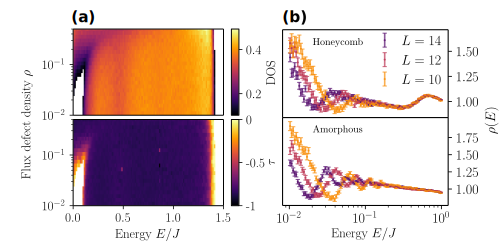
\includegraphics[width=1.\textwidth]{figs/figure_3_bashed}
    \caption{\textbf{(a)} {\color{red} Emphasize that these results are for the CSL. The topologically trivial phase should remain gapped} Density of states (top) and inverse participation ratio scaling exponent (bottom) of the fermionic spectrum as a function of flux defect density, $\tau$. Each pixel is averaged over 10 independent lattice realisations, in flux sectors sampled from an ensemble with a proportion $\rho$ of the Wilson loops flipped with respect to the ground state. White pixels correspond to bins containing no fermionic states. At low defect density, the fermionic spectra are gapped. As the defect density increases, in-gap states appear with a small $\tau$, indicating that they are strongly localized around defects. At large defect density, $\tau$ increases for the in-gap sites, indicating that they are delocalized and the system has become metallic. Using defect density as a proxy for temperature, this demonstrates the thermal phase transition from a chiral spin liquid to a thermal metal phase. \textbf{(b)} Histogrammed fermionic density of states sampled from the thermodynamic ensemble of flux sectors for $T\to\infty$, i.e. all gauge configurations equally likely. The oscillations at low $E$ are characteristic of a thermal metal phase~\cite{selfThermallyInducedMetallic2019}, demonstrated for the Kitaev honeycomb lattice model subject to a magnetic field (top) and the amorphous Kitaev model (bottom). $L$ corresponds to the linear extent of the system --- $L\sim\sqrt{N}$ with $N$ sites --- for both lattice types.}
    \label{fig:DOS_Oscillations}
\end{figure*}

{\it Anderson Transition to a Thermal Metal ---} 
An Ising non-Abelian anyon is formed by Majorana zero-modes bound to a topological defect \cite{Beenakker2013}. Interactions between anyons are modeled by pairwise projectors whose strength absolute value decays exponentially with the separation between the particles, and whose sign oscillates in analogy to RKKY exchanges \cite{Laumann2012,Lahtinen_2011,lahtinenTopologicalLiquidNucleation2012}. Disorder can induce a finite density of anyons whose hybridization lead to a macroscopically degenerate state known as \emph{thermal metal} \cite{Laumann2012}. One instance of this phase can be settled on the Kitaev CSL. In this case, the topological defects correspond to the $W_p \neq +1$ fluxes, which naturally emerge from thermal fluctuations at nonzero temperature \cite{selfThermallyInducedMetallic2019}.  \par
We demonstrated that the amorphous CSL undergoes the same form of Anderson transition by studying its properties as a function of disorder. Unfortunately, we could not perform a complete study of its properties as a function of the temperature as it was not feasible to evaluate an ever-present boundary condition dependent factor \cite{pedrocchiPhysicalSolutionsKitaev2011,Zschocke_Physical_states2015} for random networks. Instead, we evaluated the fermionic density of states (DOS) and the IPR as a function of the vortex density $\rho$ as a proxy for temperature. This approximation is exact in the limits $T = 0$ (corresponding to $\rho = 0$) and $T \to \infty$ (corresponding to $\rho = 0.5$). At intermediate temperatures the method neglects to include the influence of defect-defect correlations. However, such an approximation is enough to show the onset of low-energy excitations for $\rho \sim 10^{-2}-10^{-1}$, as displayed on the top graphic of \ref{fig:DOS_Oscillations}(a). We characterized these gapless excitations using the dimensional scaling exponential $\tau$ of the IPR on the bottom graphic of the same figure. At small $\rho$, the states populating the gap possess $\tau\approx0$, indicating that they are localised states pinned to the defects, and the system remains insulating. At large $\rho$, the in-gap states merge with the bulk band and become extensive, closing the gap, and the system transitions to a metallic phase. {\color{red} Maybe being a bit more quantitative about $\tau$ can enrich the discussion by allowing us to discuss a bit about the multifractality of these low-energy states}  \par
The thermal metal DOS displays a logarithmic divergence at zero energy and characteristic oscillations at small energies. \cite{bocquet_disordered_2000, selfThermallyInducedMetallic2019}. These features were indeed observed by the averaged density of states in the $\rho = 0.5$ case shown in \cref{fig:DOS_Oscillations}(b) for amorphous lattice. We emphasize that the CSL studied here emerges without an applied magnetic field as opposed to the CSL on the honeycomb lattice studied in Ref. \cite{selfThermallyInducedMetallic2019} {\color{red} I have the impression that \cref{fig:DOS_Oscillations}(b) on the top is very similar to Fig. 3 of \cite{selfThermallyInducedMetallic2019}. Maybe a more instructive figure would be the DOS of the amorphous toric code at the infinite temperature limit. In this case, the lack of non-Abelian anyons would be reflected by a gap on the DOS, which would contrast nicely to the thermal metal phase} \par

% This high temperature phase of the amorphous model is known as a thermal metal. The signature of the thermal metal phase is characteristic oscillations in the low energy density of states, as seen in~\cref{fig:DOS_Oscillations}(b).

{\it Discussion and Conclusions --- }
We have studied an extension of the Kitaev honeycomb model to amorphous lattices with coordination number $z= 3$. We found that it is able to support two quantum spin liquid phases that can be distinguished using a real-space generalisation of the Chern number. The presence of odd-sided plaquettes on these lattices let to a spontaneous breaking of time reversal symmetry, leading to the emergence of a chiral spin liquid phase. Furthermore we found evidence that the amorphous system undergoes an Anderson transition to a thermal metal phase, driven by the proliferation of vortices with increasing temperature. The next step is to search for an experimental realisation in amorphous Kitaev materials, which can be created from crystalline ones using several methods \cite{Weaire1976,Petrakovski1981,Kaneyoshi2018}. \par
Following the evidence for an induced chiral spin liquid phase in crystalline Kitaev materials \cite{Kasahara2018,Yokoi2021,Yamashita2020,Bruin2022}, it would be interesting to investigate if a similar state is produced on its amorphous counterpart. Besides the usual half-quantized signature on thermal Hall effect \cite{Kasahara2018,Yokoi2021,Yamashita2020,Bruin2022}, such a CSL could be also characterized using local probes such as spin-polarized scanning-tunneling microscopy \cite{Feldmeier2020,Konig2020,Udagawa2021}. The same probes would also be useful to manipulate non-Abelian anyons  \cite{Pereira2020}, thereby implementing elementary operations for topological quantum computation. Finally, the thermal metal phase can be diagnosed using bulk heat transport measurements \cite{Beenakker2013}.\par     
This work can be generalized in several ways. Introduction of symmetry allowed perturbations on the model \cite{Rau2014,Chaloupka2010,Chaloupka2013,Chaloupka2015,Winter2016}. Generalizations to higher-spin models in random networks with different coordination numbers \cite{Baskaran2008,Yao2009,Nussinov2009,Yao2011,Chua2011,Natori2020,Chulliparambil2020,Chulliparambil2021,Seifert2020,WangHaoranPRB2021,Wu2009}


% In the present work, we have avoided the need for a rigorous Monte Carlo study of the thermal phase transition. As a consequence, the thermodynamic nature of the transition between the chiral QSL and thermal metal states has not been elucidated. {\color{red} insert some guff about the Imri-Ma argument}.

{\color{red} Probably one way to make this theory experimentally relevant is to do experiments on amorphous phases of Kitaev materials. These phases can be obtained by liquifying the material and cooling it fast. Apparently, most of crystalline magnets can be transformed into amorphous ones through this process.
}
%Metal-organic frameworks (MOFs) are a promising candidate for realising Kitaev physics in an amorphous system. Yamada et al. propose a realisation of the Kitaev honeycomb model in a crystalline Ru-oxalate MOF~\cite{yamadaDesigningKitaevSpin2017}, and Misumi et al.~have demonstrated potential signatures of a resonating valence bond quantum spin liquid state in MOFs with Kagome geometry~\cite{misumiQuantumSpinLiquid2020}. Amorphous MOFs can be generated by introducing disorder into crystalline MOFs through mechanical processes~\cite{bennettAmorphousMetalOrganic2014}, suggesting a natural route to realising amorphous Kitaev physics. Assuming it is possible to realise Kitaev physics in a crystalline MOF, it is unclear what superexchange couplings would be retained when disorder is introduced to the lattice. Because it is unlikely one would cleanly reproduce the exact model described in the present work, future work should examine how robust the CSL ground state of the amorphous Kitaev model is to additional disorder in the Hamiltonian, for example random recoloring of the bonds, additional bond forming and breaking, and disorder in coupling strengths.




\bibliography{refs}% Produces the bibliography via BibTeX.
% \clearpage

\appendix

\section{Lattice Generation} \label{apx:lattice_construction}

A random pointset is used to partition space into polyhedral volumes enclosing the region closest to each point in the set. In two dimensions, the vertices and edges of these polygons form a tri-coordinate lattice.






% \section{Honeycomb lattice model}


% The Kitaev honeycomb lattice model (HLM) is composed of spin-\(\frac{1}{2}\) particles interacting anisotropically along the edges of a lattice:
% \begin{equation}
% \mathcal{H} = -\sum_{(i,j)}J^{\alpha_{ij}}\sigma_i^{\alpha_{ij}}\sigma_j^{\alpha_{ij}} + \kappa\sum_{(i,j,k)}\sigma_i^{x}\sigma_j^{y}\sigma_k^{z}
% \end{equation}
% where the two spin term runs over pairs of nearest neighbours and the three spin term runs over consecutive triplets around a plaquette. The Pauli matrices $\sigma^\alpha$ in each term are chosen according to the type, or `coloring', of the bond $i\to j$, $\alpha_{ij}\in\{x,y,z\}$. The bond coloring is chosen such that exactly one bond of each type is connected to each vertex.
% This Hamiltonian is exactly solvable by introducing a Majorana representation \(\widetilde{\sigma}_i^{\alpha} = i b^{\alpha}_i c_i\) which the partitions the Hilbert space into a classical $\mathrm{Z}_2$ gauge degree of freedom, \(u_{jk} = ib_j^{\alpha_{jk}}b_k^{\alpha_{jk}}\), on the bonds, and Majorana fermions, $c_j$, living on the vertices. It also doubles the size of the Fock space, necessitating calculating a projector \(P\) from the Majorana Fock space \(\mathcal{\widetilde{M}}\) onto the physical subspace \(\mathcal{M}\)~\cite{pedrocchiPhysicalSolutionsKitaev2011}. We refer to a choice of gauge configuration, $\{u_{jk}\}$, as the `flux sector'. The problem then reduces to solving a free-fermion Hamiltonian within each flux sector \(u\)
% \begin{equation}
% \mathcal{\widetilde{H}}^u = \frac{i}{4}\sum_{j,k}A_{jk}c_jc_k
% \end{equation}
% where $A_{jk}=2J^\alpha_{jk}u_{jk}$ for $(j, k)$ nearest-neighbours, $A_{jk}=2\kappa\sum_l u_{jl}u_{kl}$ for $(j,k)$ second-nearest-neighbours, and $A_{jk}=0$ otherwise. Finally the Majorana modes can be found with a transformation \(Q\)
% \begin{equation}
%     (b^{'}_1, b^{''}_1, ... \;b^{'}_N, b^{''}_N) = (c_1, c_2, ... \;c_{2N}) Q
% \end{equation}
% from which we create the fermionic operators \(a_i = \tfrac{1}{2} (b^{'}_i + ib^{''}_i)\), bringing \(H\) to the form
% \begin{equation}
%     \mathcal{\widetilde{H}}^u = \sum_m \epsilon_m (n_m - \tfrac{1}{2})
% \end{equation}
% with ground state energy \(E_0 = -\tfrac{1}{2}\sum_m \epsilon_m\). The projector has the effect of removing many body states with either even or odd parity \(\pi = \prod_i (1 - 2n_i)\), an effect which typically leads to a correction of order \(\tfrac{1}{N}\). The gauge symmetries of $\{u_{jk}\}$ can be removed by defining plaquette operators \(P_i = \prod_{(i,j) \in P_i} u_{ij}\) that wind the plaquettes (faces) of the lattice. 

% The ground state flux sector of the HLM in the isotropic phase ($J^x = J^y = J^z$) at zero field ($\kappa=0$) possesses a gapless fermionic spectrum. A non-zero field ($\kappa\neq0$) opens a gap, and the resulting fermionic insulator is known to host non-Abelian anyonic excitations and possess a non-zero Chern number~\cite{kitaevAnyonsExactlySolved2006}. This non-abelian phase has been shown to undergo a finite-temperature phase transition to a so-called `thermal metal' phase, which exhibits multifractility~\cite{selfThermallyInducedMetallic2019}.


\section{Euler Equation and Gauge Degeneracy}
For a lattice with \(B\) bonds, \(V\) vertices, \(P\) plaquettes and Euler characteristic \(\xi\) (0 for the torus) the Euler equation states that \(B = P + V + \xi\). This corresponds to the \(2^{B}\) gauge configurations being composed of \(2^{P - 1}\) physically distinct vortex states each of which is composed of \(2^{V - 1}\) gauge equivalent states that correspond to flipping three \(u_{ij}\) around a vertex, along with \(2 - \xi\) non-contractible loop operators. The term \(2 - \xi\) is perhaps more easily understood by relating \(\xi\) to the genus of the surface \(g\), i.e the number of holes with \(\xi = 2 - 2g\) showing that there are two non-contractible loops for each hole in the surface. 

\section{Open boundary conditions}
Care must be taken in the definition of open boundary conditions, simply removing bonds from the lattice leaves behind unpaired \(b^\alpha\) operators that need to be paired in some way to arrive at fermionic modes. In order to fix a pairing we always start from a lattice defined on the torus and generate a lattice with open boundary conditions by defining the bond coupling \(J^{\alpha}_{ij} = 0\) for sites joined by bonds \((i,j)\) that we want to remove. This creates fermionic zero modes \(u_ij\) associated with these cut bonds which we set to 1 when calculating the projector. 

\section{The Projector} \label{apx:projector}
{\color{red} Add brief mention of fermions and many body ground state}
Closely following the derivation of~\cite{pedrocchiPhysicalSolutionsKitaev2011} we can extend to the amorphous case relatively simply. The main quantity needed is the product of the local projectors \(D_i\)
\[\prod_i^{2N} D_i = \prod_i^{2N} b^x_i b^y_i b^z_i c_i \]
for a lattice with \(2N\) vertices and \(3N\) edges. The operators can be ordered by bond type without utilising any property of the lattice.
\[\prod_i^{2N} D_i = \prod_i^{2N} b^x_i \prod_i^{2N} b^y_i \prod_i^{2N} b^z_i \prod_i^{2N} c_i\]
The product over \(c_i\) operators reduces to a determinant of the Q matrix and the fermion parity. The only problem is to compute the factors \(p_x,p_y,p_z = \pm1\) that arise from reordering the b operators such that pairs of vertices linked by the corresponding bonds are adjacent.
\[\prod_i^{2N} b^\alpha_i = p_\alpha \prod_{(i,j)}b^\alpha_i b^\alpha_j\]
This is simple the parity of the permutation from one ordering to the other and can be computed easily with a cycle decomposition.

The final form is almost identical to the honeycomb case with the addition of the lattice structure factors \(p_x,p_y,p_z\)
\[P^0 = 1 + p_x\;p_y\;p_z \mathrm{det}(Q^u) \; \hat{\pi} \; \prod_{\{i,j\}} -iu_{ij}\] 

\(\mathrm{det}(Q^u)\) is the determinant of the matrix that takes \((c_1, c_2... c_{2N}) Q = (b_1, b_2... b_{2N})\). This along with \(\prod u_{ij}\) depend on the lattice and the particular vortex sector. 

\(\hat{\pi} = \prod{i}^{N} (1 - 2\hat{n}_i)\) is the parity of the particular many body state determined by fermionic occupation numbers \(n_i\). The Hamiltonian is \(H = \sum \epsilon_i (n_i - 1/2)\) in this basis and this tells use that the ground state is either an empty system with all \(n_i = 0\) or a state with a single fermion in the lowest level. 

\section{Numerical Evidence for the Ground State Flux Sector} \label{apx:ground_state}

In this section we detail the numerical evidence collected to support the claim that, for an arbitrary lattice, a gapped ground state flux sector is found by setting the flux through each plaquette to $\phi_{\textup{g.s.}} = -(\pm i)^{n_{\textup{sides}}}$. This was done by generating a large number ($\sim$ 25,000) of lattices and exhaustively checking every possible flux sector to find the configuration with the lowest energy. We checked both the isotropic point ($J^\alpha = 1$), as well as in the toric code phase ($J^x = J^y = 0.25, J^z = 1$).\par 
The argument has one complication: for a graph with $n_p$ plaquettes, there are $2^{n_p - 1}$ distinct flux sectors to search over, with an added factor of 4 when the global fluxes $\Phi_x$ and $\Phi_y$ are taken into account. Note that the $-1$ appears in this counting because fluxes can only be flipped in pairs. To be able to search over the entire flux space, one is necessarily restricted to looking at small system sizes -- we were able to check all flux sectors for systems with $n_p \leq 16$ in a reasonable amount of time. However, at such small system size we find that finite size effects are substantial enough to destroy our results. In order to overcome these effects we tile the system and use Bloch's theorem (a trick that we shall refer to as \textit{twist-averaging} for reasons that shall become clear) to efficiently find the energy of a much larger (but periodic) lattice. Thus we are able to suppress finite size effects, at the expense of losing long-range disorder in the lattice.\par
Our argument has three parts: First we shall detail the techniques used to exhaustively search the flux space for a given lattice. Next, we discuss finite-size effects and explain the way that our methods are modified by the twist-averaging procedure. Finally, we demonstrate that as the size of the disordered system is increased, the effect of twist-averaging becomes negligible -- suggesting that our conclusions still apply in the case of large disordered lattices. 

{\it Testing All Flux Sectors ---}
For a given lattice and flux sector, defined by $\{ u_{jk}\}$, the fermionic ground state energy is calculated by taking the sum of the negative eigenvalues of the matrix
\begin{align}
    M_{jk} = \frac{i}{2} J^{\alpha} u_{jk}.
\end{align}
The set of bond variables $u_{jk}$, which we are free to choose, determine the $\mathbb Z_2$ gauge field. However only the fluxes, defined for each plaquette according to eqn.~\ref{eqn:flux_definition}, have any effect on the energies. Thus, there is enormous degeneracy in the $u_{jk}$ degrees of freedom. Flipping the bonds along any closed loop on the dual lattice has no effect on the fluxes, since each plaquette has had an even number of its constituent bonds flipped - as is shown in the following diagram:
\begin{center}
    \input{tikzpictures/flux_loop}
\end{center}
where the flipped bonds are shown in red. In order to explore every possible flux sector using the $u_{jk}$ variables, we restrict ourselves to change only a subset of the bonds in the system. In particular, we construct a spanning tree on the dual lattice, which passes through every plaquette in the system, but contains no loops. 
\begin{center}
    \input{tikzpictures/spanning_tree}
\end{center}
The tree contains $n_p - 1$ edges, shown in red, whose configuration space has a $1:1$ mapping onto the $2^{n_p - 1}$ distinct flux sectors. Each flux sector can be created in precisely one way by flipping edges only on the tree (provided all other bond variables not on the tree remain fixed). Thus, all possible flux sectors can be accessed by iterating over all configurations of edges on this spanning tree.

\begin{figure*}[t]
    \centering
    \includegraphics[width=\textwidth]{figs/appendix_diagram.png}
    \caption{(a) The energy of every flux sector explored for a system of 16 plaquettes, the order is arbitrary. The two ground state flux sectors can be identified as the points with lowest energy. (b) The fermion gap for each of the flux sectors explored. Note that the largest fermion gap coincides with the ground state flux sector. This occurred in $\sim 85\%$ of cases tested. (c) Average energy of the systems tested over a range of system sizes from $n_p$ = 9 to $n_p = 1600$. The region between the upper and lower quartiles is shown in red, and the full range of energies obtained is shown in orange. (d) Average fermion gap as a function of system size. Again, the region between the upper and lower quartiles is shown in red, and the full range is shown in orange. As can be seen, no gapless systems were found for $n_p > 20$. }
    \label{fig:energy_gaps_example}
\end{figure*}

{\it Finite Size Effects ---}
In our numerical investigation, the objective was to test as many example lattices as possible. We aim for the largest lattice size that could be efficiently solved, requiring a balance between lattice size and cases tested. Each added plaquette doubles the number of flux sectors that must be checked. 25,000 lattices containing 16 plaquettes were used. However, in his numerical investigation of the honeycomb model, Kitaev demonstrated that finite size effects persist up to much larger lattice sizes than we were able to access \cite{kitaevAnyonsExactlySolved2006}. \par 
In order to circumvent this problem, we treat the 16-plaquette amorphous lattice as a unit cell in an arbitrarily large periodic system. The bonds that originally connected across the periodic boundaries now connect adjacent unit cells. This infinite periodic Hamiltonian can then be solved using Bloch's theorem, since the larger system is diagonalised by a plane wave ansatz. For a given crystal momentum $\bf q \in [0,2\pi)^2 $, we are left with a Bloch Hamiltonian, which is identical to the original Hamiltonian aside from an extra phase on edges that cross the periodic boundaries in the $x$ and $y$ directions,
\begin{align}
    M_{jk}(\bf q) =  \frac{i}{2} J^{\alpha} u_{jk} e^{i q_{jk}},
\end{align}
where $q_{jk} = q_x$ for a bond that crosses the $x$-periodic boundary in the positive direction, with the analogous definition for $y$-crossing bonds. We also have $q_{jk} = -q_{kj}$. Finally $q_{jk} = 0$ if the edge does not cross any boundaries at all -- in essence we are imposing twisted boundary conditions on our system. The total energy of the tiled system can be calculated by summing the energy of $M(\bf q)$ for every value of $\bf q$. In practice we constructed a lattice of $50 \times 50$ values of $\bf q$ spanning the Brillouin zone. The procedure is called twist averaging because the energy-per-unit cell is equivalent to the average energy over the full range of twisted boundary conditions. \par 
{\it Evidence for the Ground State Ansatz ---}
For each lattice with 16 plaquettes, $2^{15} =$ 32,768 flux sectors are generated. In each case we find the energy (averaged over all twist values) and the size of the fermion gap, which is defined as the lowest energy excitation for any value of $\bf q$. We then check if the lowest energy flux sector aligns with our ansatz (eqn.~\ref{eqn:gnd_flux}) and whether this flux sector is gapped. \par
In the isotropic case ($J^\alpha = 1$), all 25,000 examples conformed to our guess for the ground state flux sector. A tiny minority ($\sim 10$) of the systems were found to be gapless. As we shall see shortly, the proportion of gapless systems vanishes as we increase the size of the amorphous lattice. An example of the energies and gaps for one of the systems tested is shown in fig.~\ref{fig:energy_gaps_example}. For the anisotropic phase (we used $ J^x, J^y = 0.25, J^z = 1$) the overwhelming majority of cases adhered to our ansatz, however a small minority ($\sim 0.5 \%$) did not. In these cases, however, the energy difference between our ansatz and the ground state was at most of order $10^{-6}$. Further investigation would need to be undertaken to determine whether these anomalous systems are a finite size effect due to the small amorphous system sizes used or a genuine feature of the toric code phase on such lattices. \par

{\it A Gapped Ground State ---} Now that we have collected sufficient evidence to support our guess for the ground state flux sector, we turn our attention to checking that this sector is gapped. We no longer need to exhaustively search over flux space for the ground state, so it is possible to go to much larger system size. We generate 40 sets of systems with plaquette numbers ranging from 9 to 1600. For each system size, 1000 distinct lattices are generated and the energy and gap size are calculated without phase twisting, since the effect is negligible for such large system sizes. As can be seen, for very small system size a small minority of gapless systems appear, however beyond around 20 plaquettes all systems had a stable fermion gap in the ground state. 

% Thus, we shall begin with a discussion of how finite size affects the eigenvalues of the Majorana Hamiltonian, followed by our solution to this problem. Evidence for the ground state solution was collected by searching over all possible flux sectors for the lowest energy states. This is repeated for various values of $J$ over a large number of randomly generated lattices. \par

% For a given lattice and flux sector, defined by $\{ u_{jk}\}$, the fermionic ground state energy is found by taking the sum of the negative eigenvalues of the matrix
% \begin{align}
%     M_{jk} = \frac{i}{2} J^{\alpha} u_{jk}.
% \end{align}
% A gauge transformation involves flipping the value of $u_{jk}$ for the three bonds connected to the point at $j$. Under a gauge transformation, the matrix $M$ transforms according to $M \rightarrow D_j M D_j$, where the matrix $D_j$ is a diagonal matrix with $-1$ on the $j$'th entry, and $+1$ on all others. This represents a unitary transformation, so the spectrum of $M$ is invariant under gauge transformations. As demonstrated in \cite{Lieb2004}, the spectrum is determined entirely by the flux through all circuits in the system, which we define analogously to \ref{eqn:flux_definition}. In this case we include not only plaquettes, but circuits that encircle several plaquettes. In periodic boundaries we must also consider 

% In the language of graph theory, this matrix may be interpreted as representing a weighted, directed digraph, with weights determined by the individual entries of $M$. The Harary-Sachs theorem \cite{StreifelSkewCharacteristic2016,HararyDeterminant1962} states that the characteristic polynomial of such a matrix may be written in terms of the weights of the cycles of the graph, defined as the product of the elements of $M$ around some closed path $\mathcal C$ on the lattice,
% \begin{align}
%     w_{\mathcal{C}} = \prod_{\mathcal {C}} M_{jk}.
% \end{align}
% These weights are similar to the fluxes defined in the bulk text, with two important differences. Firstly, the cyclic weights include the factor of $J^\alpha$ in the product. Secondly, unlike tthe fluxes, which are defined for individual plaquettes, the weights are  calculated for every closed path on the lattice. The takeaway is that the characteristic polynomial, and thus all eigenvalues, is determined only by the values of these weights. Any change to the set of $u_{jk}$ that does not affect the weight of any cycles will have no effect on the energies of the system. For example a gauge transformation, where $u_{jk}$ is flipped on the three edges connected to a chosen site, cannot affect the energies, as every cycle passing through the chosen site must contain two of the flipped edges. \par



\end{document}

